\section{Experiment}

Main goal: explain what you did with enough detail so the reader could reproduce it
Include the equipment used, quantities you measured (if relevant also the accuracy of the
equipment), procedures you followed
Diagrams (e.g. scheme of the circuit) can be included
Please do not include results here!




\subsection{Part 1}
During the first part of the lab we messured 


\begin{figure}[H]
    \centering    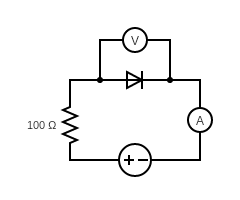
\includegraphics[width=0.3\textwidth]{Figures/circuit_part1.png}
    \caption{This figure...}
    \label{fig:part1_circuit}
\end{figure}





    
\subsection{Part 2}




\subsection{Part 3}
\begin{figure}[H]
    \centering    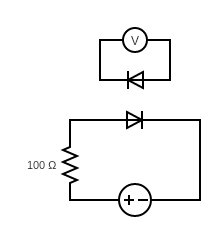
\includegraphics[width=0.3\textwidth]{Figures/circuit_part3.png}
    \caption{This figure...}
    \label{fig:part3_circuit}
\end{figure}


